% Especificaciones del tamaño de letra, tamaño de hoja, márgenes, librerias, etc.
\documentclass[12pt, letterpaper]{article}
\usepackage[english]{babel}
\usepackage{fancyhdr}
\usepackage[utf8]{inputenc}
\usepackage[T1]{fontenc}
\usepackage{amsmath}
\usepackage{graphicx}
\usepackage{subcaption}
\usepackage[hidelinks]{hyperref}
\usepackage{url}
\usepackage{amssymb}
\usepackage{float}
\usepackage[margin=1in]{geometry}
\usepackage{listings}
\usepackage{verbatim}
\renewcommand{\baselinestretch}{1.5}

% Enlace Bibliografía
\usepackage{csquotes}
\usepackage[notes,backend=biber]{biblatex-chicago}
\addbibresource{referencias.bib}

% Titulo, autores, fecha.
\title{Práctica \#2: Creación de Perfiles Alares}
\author{Carlos A. Vásquez Castañeda \and 1155057 \and Grupo 395}
\date{Febrero 29, 2020}
\pagestyle{fancy}
\fancyhf{}
\rhead{Mecánica de Sustentación}
\lhead{Práctica \#2}
\rfoot{\thepage}


% Inicio del documento
\begin{document}
\maketitle

\section*{Introducción}
Anterior al desarrollo de perfiles alares de la series del Comité Nacional Asesor para la Aeronáutica (NACA), el diseño de los perfiles era más arbitrario sin alguna guía para el diseñador a excepción de la experiencia previa poseída, experimentaciones con modificaciones de formas ya diseñadas y datos adquiridos mediante pruebas.

A principios de los años 1930 la metodología para el diseño de perfiles alares cambió gracias a una publicación de un reporte de la NACA titulado "Las características de 78 perfiles relacionados de pruebas en el túnel de viento de densidad variable". En este reporte, los autores notaron que había muchas similitudes entre los perfiles que fueron los más exitosos, que las dos primeras variables que afectan estas geometrías son la pendiente de la línea de combadura media y la distribución de espesores abajo y arriba de esta línea. Entonces, a partir de estas variables, desarrollaron una serie de ecuaciones que podían ser utilizadas para generar una familia completa de formas de perfil relacionadas.

Así, el diseño de perfiles alares se volvió más sofisticado, y de estas primeras aproximaciones actualmente se han hecho modificaciones, sin embargo las variables principales de las que hablábamos anteriormente seguían presentes en estas ecuaciones, como se muestra en la siguiente figura.

\begin{figure}[H]
	\centering
	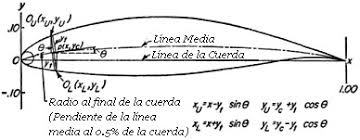
\includegraphics[width=\textwidth]{ay.jpeg}
	\caption{Construcción geométrica del perfil NACA.}
\end{figure}

La primera familia de perfiles diseñados utilizando estas ecuaciones se conoció como la serie NACA de 4 dígitos. El primer dígito especifica la combadura máxima (m) en porcentaje de la cuerda (longitud del perfil), el segundo indica la posición de la combadura máxima (p) en décimas de cuerda, y los dos últimos números indican el espesor máximo (t) del perfil en porcentaje de la cuerda. Como ejemplo, analicemos el perfil NACA 2415. Este perfil tiene un espesor máximo del 15\% con una combadura máxima del 2\% localizada al 40\% detrás del borde de ataque de perfil.

Existen más clasificaciones de los perfiles NACA, entre las cuales se encuentran las siguientes:

\begin{itemize}
	\item Seria NACA de 5 dígitos.
	\item Serie NACA de 4 y 5 dígitos modificada.
	\item Serie NACA 1 o NACA 16.
	\item Serie NACA 6.
	\item Serie NACA 7.
	\item Serie NACA 8.
\end{itemize}

\noindent Cada una cuenta con distintas caracterísitcas y logros obtenidos.

Como último punto a tratar, las funciones a trozos presentan una gran versatilidad en el modelado de ecuaciones. Sin restringirnos a una función definida por una sola ecuación, es más sencillo su utilización. Si no utilizaramos estas herramientas probablemente tendríamos que utilizar series de Taylor,  Maclaurin o curvas de Bézier para lograr un modelado aproximado de una región del perfil, lo cual aumentaría el grado del polinomio utilizado y no sería completamente distinguible dónde inicio y acaba el perfil alar. Es por esto que las funciones a trozos son de gran utilidad.

\section*{Procedimiento de la Práctica}
El objetivo final de la práctica es encontrar una ecuación que modele la comba del perfil alar NACA de 4 dígitos, para cualquier valor arbitrario de comba. Para esto utilizaremos el siguiente sistema de ecuaciones.

\begin{equation}
	z_{cam}(x) = 
	\left\{
	\begin{array}{ll}
		b_0 + b_1 x + b_2 x^2 & x \in [0, x_{mc}] \\
		b_3 + b_4 x+ b_5 x^2 & x \in [x_{mc}, 1] \\
	\end{array}
	\right.
\end{equation}

Este sistema cuenta con las siguientes condiciones:
\begin{itemize}
	\item Las condiciones de los puntos extremos $z_{cam}(0) = 0$ y $z_{cam}(1) = 0$.
	\item Las condiciones de combadura máxima $\frac{dz_{cam}}{dx}\Bigr|_{\substack{x=x_{mc}}} = 0$ y $z_{cam}(x_{mc}) = z_{cam}^{max}$.
\end{itemize}

Para obtener una solución general podemos realizar un análisis mediante Wolfram Mathematica de la siguiente manera.

\begin{figure}[H]
	\centering
	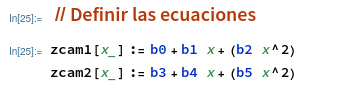
\includegraphics[width=\textwidth]{1.png}
	\caption{Se define el sistema de ecuaciones que se presentó con anterioridad.}
\end{figure}

\begin{figure}[H]
	\centering
	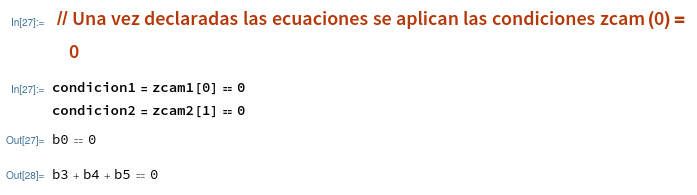
\includegraphics[width=\textwidth]{2.png}
	\caption{Condiciones de los puntos extremos se definen.}
\end{figure}
Como podemos observar en la figura 3, a partir de las primeras ecuaciones y condiciones es posible ya obtener una constante de entre las seis. Sin embargo, a partir de los principio del álgebra lineal, si contamos con estas 6 incógnitas, no nos será posible obtener todas las incógnitas a menos que contemos con seis ecuaciones que las relacionen mutuamente. es por eso que ahora debemos definir las condiciones de combadura.

\begin{figure}[H]
	\centering
	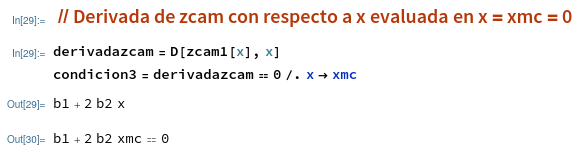
\includegraphics[width=\textwidth]{3.png}
	\caption{Definición de las condiciones de combadura.}
\end{figure}

\begin{figure}[H]
	\centering
	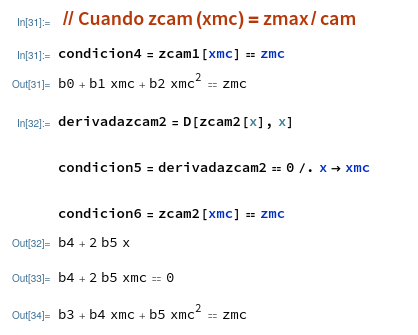
\includegraphics[width=\textwidth]{4.png}
	\caption{Últimas condiciones, éstas se obtienen a partir de condiciones básicas de cálculo diferencial (puntos de inflexión y máximos y mínimos).}
\end{figure}

\begin{figure}[H]
	\centering
	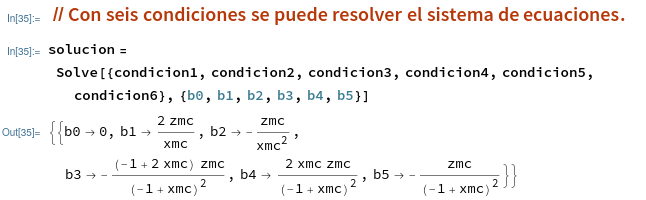
\includegraphics[width=\textwidth]{5.png}
	\caption{Resolución del sistema de ecuaciones.}
\end{figure}

Una vez obtenidas los valores de las incógnitas $b_0 \hdots b_5$ reemplazamos len las ecuaciones originales los valores de la solución para obtener las dos partes de la ecuación que definirá la combadura.

\begin{figure}[H]
	\centering
	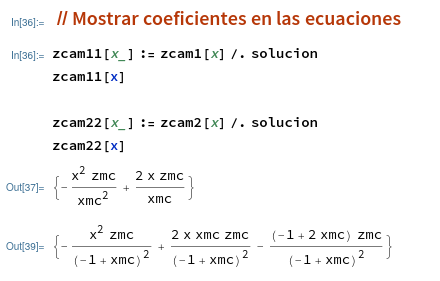
\includegraphics[width=0.8\textwidth]{6.png}
	\caption{Reemplazo de los valores $b_0 \hdots b_5$.}
\end{figure}

\begin{figure}[H]
	\centering
	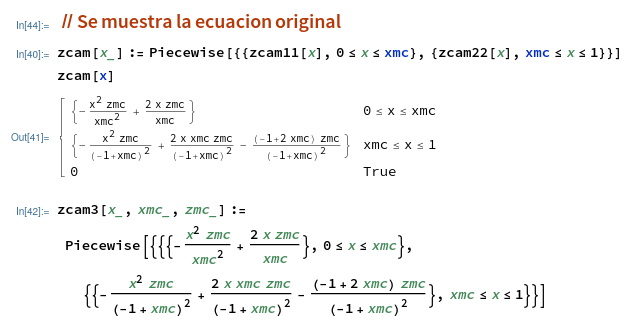
\includegraphics[width=\textwidth]{7.png}
	\caption{Unión de la ecuación original en una función a trozos.}
\end{figure}

En la figura 8 se muestra la unión de la función a trozos (en $In[40]$), sin embargo esta función definida tiene las variables $x_{mc}$ y $z_{mc}$. Esto es correcto debido a que hemos hallado una expresión general para cualquier $x_{mx}$ y $z_{mc}$, por lo que posteriormente definimos una ecuación llamada $z_{cam_3}$, la cual nos permite otorgarle cualquier valor a las variables en cuestión.

\begin{figure}[H]
	\centering
	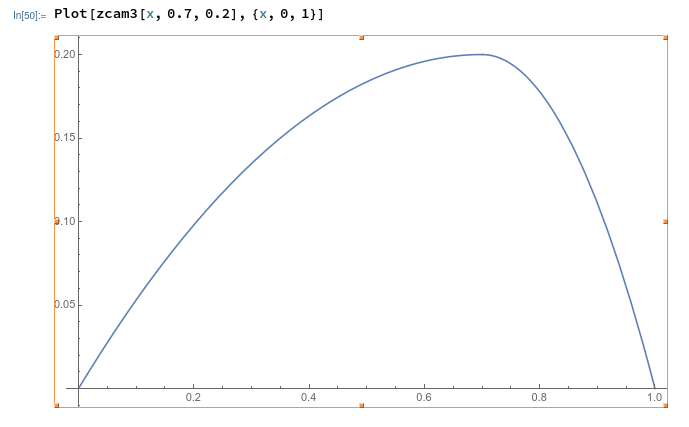
\includegraphics[width=\textwidth]{8.png}
	\caption{Gráfica de la parte superior del perfil con una $x_{mc} = 0.7$ y una $z_{cam}^{cam} = 0.2$.}
\end{figure}

\section*{Conclusión}
El modelado de perfiles alares mediante la metodología NACA permite la estandarización de los perfiles alares. Estas soluciones analíticas son de gran utilidad ya que posteriormente si se desea realizar un análisis en alguna de sus propiedades geométricas resultará más sencillo contar con la ecuación como tal para la aplicación de operadores lineales que nos permitan conocer estos datos.

A pesar de necesitar un procedimiento un poco extenso para la definición de la curva, es de gran utilidad ya que si deseamos un perfil alar con las mismas caracterísitcas pero con un parámetro de combadura diferente, nos será posible la modificación de éste si modificamos un sólo valor en la función.

En conclusión, al utilizar las ecuaciones, la ecuación obtenida permitirá el modelado de modelos mucho más sofisticados que nos permitan analizar otras propiedades, ya sean geométricas o físicas mediante la discretización de la curva.
%%%%%  Bib
\renewcommand\refname{References}
\printbibliography
\end{document}
